\documentclass[a4paper,11pt]{book}
\usepackage[francais]{babel}
\usepackage[table]{xcolor}
\usepackage{amsmath}
\usepackage[utf8]{inputenc}
\usepackage{textcomp}
\usepackage{gensymb}
%\usepackage[francais]{babel}
\usepackage[T1]{fontenc}
\usepackage{makeidx}
\usepackage{graphicx}
\usepackage{enumitem}
\usepackage{float}
\usepackage{relsize}
\usepackage{amsmath,amsfonts,amssymb}
\usepackage{multirow}
\usepackage{layout}
\usepackage{amsthm}
\usepackage{lmodern}
\usepackage{fancyhdr}
\usepackage{enumitem}
\usepackage{geometry}
\usepackage{listings}
\definecolor{darkWhite}{rgb}{0.94,0.94,0.94}

\lstdefinestyle{generalFrame}{
aboveskip=3mm,
belowskip=-2mm,
basicstyle=\footnotesize,
breakatwhitespace=false,
breaklines=true,
captionpos=b,
commentstyle=\color{red},
deletekeywords={...},
escapeinside={\%*}{*)},
extendedchars=true,
framexleftmargin=16pt,
framextopmargin=3pt,
framexbottommargin=6pt,
frame=tb,
keepspaces=true,
keywordstyle=\color{blue},
language=Python,
literate=
{²}{{\textsuperscript{2}}}1
{⁴}{{\textsuperscript{4}}}1
{⁶}{{\textsuperscript{6}}}1
{⁸}{{\textsuperscript{8}}}1
{€}{{\euro{}}}1
{é}{{\'e}}1
{è}{{\`{e}}}1
{ê}{{\^{e}}}1
{ë}{{\¨{e}}}1
{É}{{\'{E}}}1
{Ê}{{\^{E}}}1
{û}{{\^{u}}}1
{ù}{{\`{u}}}1
{â}{{\^{a}}}1
{à}{{\`{a}}}1
{á}{{\'{a}}}1
{ã}{{\~{a}}}1
{Á}{{\'{A}}}1
{Â}{{\^{A}}}1
{Ã}{{\~{A}}}1
{ç}{{\c{c}}}1
{Ç}{{\c{C}}}1
{õ}{{\~{o}}}1
{ó}{{\'{o}}}1
{ô}{{\^{o}}}1
{Õ}{{\~{O}}}1
{Ó}{{\'{O}}}1
{Ô}{{\^{O}}}1
{î}{{\^{i}}}1
{Î}{{\^{I}}}1
{í}{{\'{i}}}1
{Í}{{\~{Í}}}1,
morekeywords={*,...},
numbers=none,
numbersep=10pt,
numberstyle=\tiny\color{black},
rulecolor=\color{black},
showspaces=false,
showstringspaces=false,
showtabs=false,
stepnumber=1,
stringstyle=\color{gray},
tabsize=4,
title=\lstname,
}

\definecolor{darkseagreen}{rgb}{0.56, 0.74, 0.56}
\definecolor{darkpastelblue}{rgb}{0.47, 0.62, 0.8}

\lstnewenvironment{mypython}
  {\lstset{language=python,
  style =generalFrame,
  backgroundcolor=\color{darkWhite} }}
  {}

\lstnewenvironment{mybash}
  {\lstset{language=python,
  	style=generalFrame,
	backgroundcolor=\color{darkseagreen} }}
  {}

\lstnewenvironment{myoutput}
  {\lstset{language=bash,
  	style=generalFrame,
	backgroundcolor=\color{darkpastelblue} }}
  {}


\geometry{hmargin=2.2cm,vmargin=2.9cm}

 
\pagestyle{fancy}
\fancyhf{}
\fancyhead[L]{\leftmark}
\fancyfoot[C]{\thepage}
    
\theoremstyle{theo}
%\newtheorem{thm}{Theorem}

\newtheorem{theorem}{Théorème}[section]
\newtheorem{corollary}{Corollaire}[theorem]
\newtheorem{lemma}[theorem]{Lemme}
\newtheorem{prop}{Proposition}
	

\newcommand*{\QEDA}{\hfill\ensuremath{\blacksquare}}%
\newcommand*{\QEDB}{\hfill\ensuremath{\square}}%
\newcommand*{\R}{{\rm I\!R}}
\newcommand*{\Hi}{\mathcal{H}}

\newcommand\vbar[1]{\vrule\begin{tabular}[t]{l}#1\end{tabular}}
\newcommand{\bproof}{\begin{itemize} \item {\bf D\'emonstration.
\hspace{0.2cm}}}
\newcommand{\eproof}{\end{itemize}}
\usepackage[memoire]{PageDeGarde}
\def\CadreBleuhpos{500}

\def\entetehpos{-50}
\def\entetevpos{540}


%===================================
%  Fin renseignements a completer
%===================================


% ==================================================================
%               FIN TITLE PAGE 
% ==================================================================
\setlength{\headheight}{15.35403pt}
\begin{document}
\let\cleardoublepage\clearpage
\title{ \usefont{T1}{ptm}{m}{n} Tutoriel TensorFlow}

\annee{2017-2018}

\Auteur{IKNI Layachi}{}

\Encadrant{Pag\'e Vincent}{MCF à l'Université des Antilles}


\maketitle

\newpage
%\section*{Remerciements}
%\bigskip
%\pagestyle{plain}
%\bigskip
%\newpage 

\tableofcontents
\newpage
\chapter{Introduction }

\section{Installation}
TensorFlow est une librairie de calcul dédiée à l'apprentissage automatique. On peut l'utiliser avec python, java, C,.... Dans notre cas, nous utiliserons python.


Pour l'installation, nous avons suivi les instructions du tutoriel officiel qui se trouve ici, sans difficultés :

https://www.tensorflow.org/install/


\section{Premiers concepts de TensorFlow}

Tout d'abord, TensorFlow s'appuie sur des concepts de programmation très différents d'une programmation standard python. Pour bien les comprendre, prenons un exemple :


On veut que notre programme prenne une valeur réelle (x), calcule une valeur  $y = W*x+b$ avec $W$ et $b$ des valeurs réelles que notre programme sera appelé a modifier plus tard.

le code correspondant en python est le suivant
\begin{mypython}
x = 2
W = 0.3
b = -0.3
y = W*x+b
print(y)
\end{mypython}

La sortie de ce programme serait :
\begin{myoutput}
0.3
\end{myoutput}

ici, $W$, $b$ , $x$ et $y$ sont des variables du programmes.
Néanmoins, dans le contexte de notre programme, elles jouent des rôles très différents :
\begin{itemize}
\item $x$ est une entrée 
\item $W$ et $b$ sont des valeurs modifiables
\item $y$ est calculé a partir de $x$, $W$ et $b$
\end{itemize}

La programmation en TensorFlow, met en place cette différence.
\begin{itemize}
\item $x$ sera appelé un \textbf{placeholder} , (en deux mots : une variable dont on promet qu'on lui donnera une valeur au moment du run)
\item $W$ et $b$ seront définis comme des variables
\item $y$ sera défini implicitement par l'équation de calcul 
\end{itemize}

Notons qu'il existe aussi la notion de constante, non présentée ici, mais facile a appréhender.

Le code correspondant en TensorFlow est le suivant :
\begin{mypython}
import tensorflow as tf

x = tf.placeholder(tf.float32)

W = tf.Variable([.3], dtype=tf.float32)
b = tf.Variable([-.3], dtype=tf.float32)

y = W*x + b

print(y)
\end{mypython}

La sortie de ce programme est alors surprenante :
\begin{myoutput}
Tensor("add:0", dtype=float32)
\end{myoutput}

De fait, nous n'avons pas calculé la valeur de $y$.\\
En fait notre programme ne manipule pas des variables au sens traditionnel, mais explique les dépendances entres les différents éléments de notre programme (ce sont des nœuds du graphes de calcul). TensorFlow s'appuie sur ce graphe de calcul, sur lequel nous reviendrons plus tard pour comprendre son intérêt.\\

Le graphe correspondant est représenté ci-dessous pour information.
\begin{figure}[H]

\begin{center}
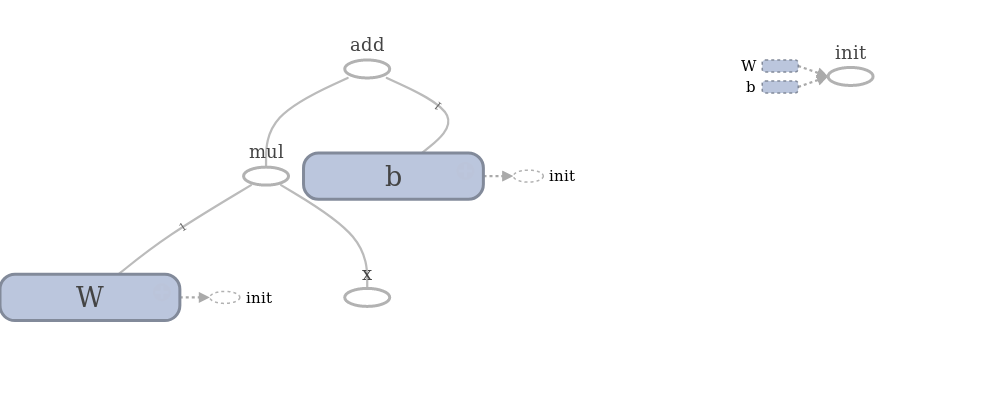
\includegraphics[width=10cm]{./figures/graph_addition.png} 
\end{center}
\caption{Graphe de calcul simple}
\end{figure}

On retrouve dans ce graphes la présence des deux variables ($W$ et $b$), le placeholder $x$, et un noeud $add$ dont la sortie correspond à $y$.


Par ailleurs, les variables au sens TensorFlow sont des nœuds de calculs qui peuvent être modifiés. Elle ne sont pas initialisées par leur déclaration. Il faudra explicitement demander leur initialisation pour qu'elles agissent comme on s'y attend.
Il s'agit maintenant pour que notre programme calcule bien la valeur voulue de :
\begin{itemize}
\item construire le graphe de calcul a partir des informations précédentes.
\item initialiser les variables $W$ et $b$
\item lancer le calcul de y avec une valeur choisie pour $x$...
\end{itemize}

Ajoutons les codes suivants à notre programme
\begin{mypython}
sess = tf.Session()
\end{mypython}
Le code ci-dessus construit le graphe.
\begin{mypython}
init = tf.global_variables_initializer()
sess.run(init)
\end{mypython}
Le code ci-dessus initialise toutes les variables du programme (W et b). En fait, ce code construit un noeud de calcul correspondant a l'initialisation (première ligne) et lance le calcul correspondant (deuxième ligne).

\begin{mypython} 
resu = sess.run(y, {x:2}) 
print(resu)
\end{mypython}
Ce code lance le calcul de y, en prenant soin de placer la valeur 2 dans le placeholder x et afficher le résultat attendu
\begin{myoutput}
[0.3]
\end{myoutput}
Pour comprendre l'intérêt de ces concepts de graphe de calcul, ajoutons à la fin de notre programme existant le code suivant :

\begin{mypython} 
resu = sess.run(y, {x:[1, 2, 3]}) 
print(resu)
\end{mypython} 

Cette fois ci, les sorties sont :

\begin{mypython} 
[0.3]
[0.  0.3 0.6]
\end{mypython} 

Nous avons en fait lancé deux runs (deux calculs de y). La première fois, x est un réel, la seconde fois x est un tableau de réels. Dans le second cas, pour chaque valeur de x, une valeur est calculée pour y.
Notre programme a donc mis en place une procédure de calcul (le graphe de calcul) que l'on peut utiliser de multiples fois, avec différentes valeurs d'entrées (qui de plus prennent des formes différentes).
Une grande partie de la force de TensorFlow tient dans ces notions.
Voici donc le code du programme complet :

\begin{mypython} 
import tensorflow as tf

x = tf.placeholder(tf.float32, name="x")

W = tf.Variable([.3], dtype=tf.float32, name="W")
b = tf.Variable([-.3], dtype=tf.float32, name="b")

y = W*x + b

print(y)

sess = tf.Session()

init = tf.global_variables_initializer()
sess.run(init)

resu = sess.run(y, {x:2}) 
print(resu)

resu = sess.run(y, {x:[1, 2, 3]}) 
print(resu)
\end{mypython} 

\section{Premiers pas avec Tensorboard}

TensorBoard est l'outil de visualisation associé à TensorFlow. Il permet de visualiser le graphe de calcul, mais aussi des valeurs importantes retenues lors des calculs exécutés sur ce graphe de calcul.
Pour sélectionner les informations a visualiser, nous l'indiquerons a notre programme TensorFlow. Le programme sauvegardera ces informations dans un répertoire spécifique.

On pourra alors lancer l'exécutable TensorBoard qui va analyser ce répertoire, créer un serveur web local que l'on pourra consulter pour visualiser nos informations...
Voyons comment tout ceci se fait.


Ajout de code dans le programme TensorFlow (a la fin du programme précédent) :
\begin{mypython}
pathLog="./pathLog/";
writer = tf.summary.FileWriter(pathLog, sess.graph)
writer.close()
\end{mypython}
Ici, on choisit le répertoire (répertoire de Log) dans lequel seront stockées les informations importantes, et on crée un objet permettant d'écrire les informations de notre programme sur le disque. Ici, nous ne sauvons que le graphe de calcul. Enfin, on ferme cet objet.
On lance notre programme TensorFlow 
\begin{mybash}
python .\premiersPas.py
\end{mybash}
On lance ensuite TensorBoard sur le répertoire de Log avec une ligne dépendant de l'OS utilisé :

Sous windows :
\begin{mybash}
tensorboard.exe --logdir=./pathLog
\end{mybash}
Sous linux :
\begin{mybash}
tensorboard --logdir=./pathLog
\end{mybash}

L’exécution donne le message suivant :
\begin{myoutput}
Starting TensorBoard b'41' on port 6006
(You can navigate to http://127.0.1.1:6006)
\end{myoutput}


Enfin, on ouvre un navigateur dans lequel on indique l'URL de consultation indiquée par la sortie précédente.

Voici une capture de la visualisation obtenue :
\begin{figure}[H]

\begin{center}
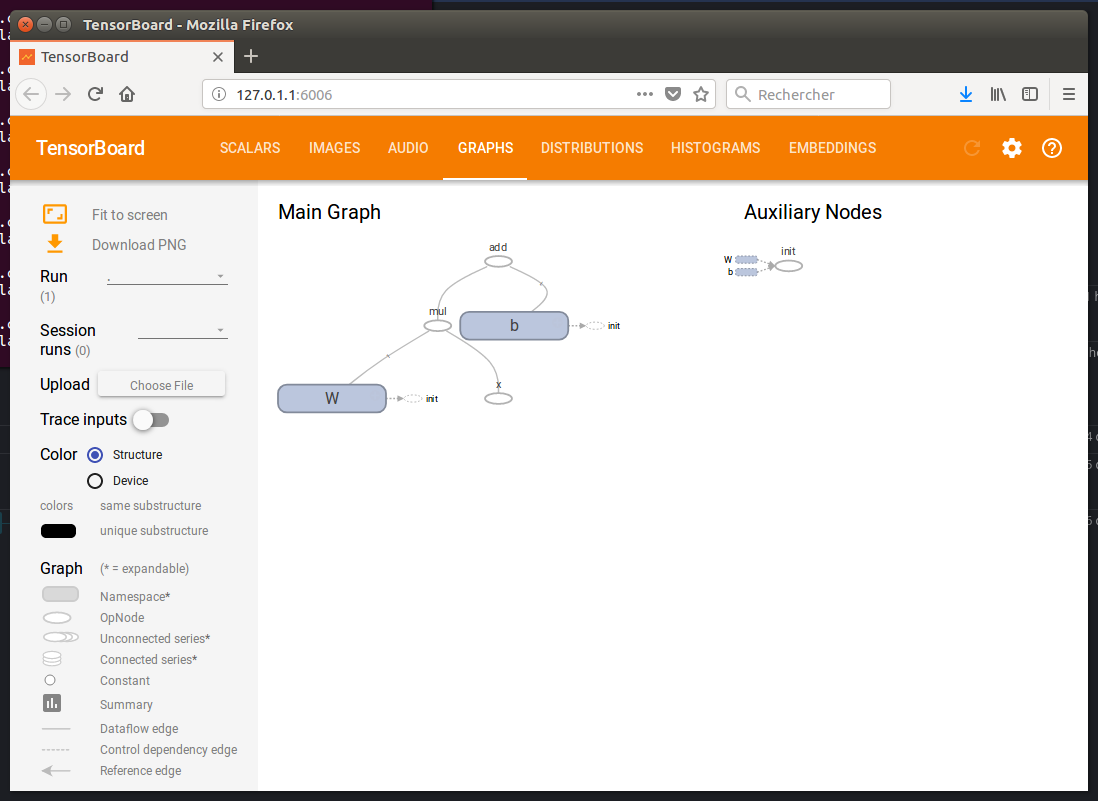
\includegraphics[width=10cm]{./figures/premierTensorFlow.png} 
\end{center}
\caption{La fenêtre de visualisation de TensorBoard}
\end{figure}

On retrouve ici le graphe précédent. Notez le sous graphe en haut a droite (noeud init) correspondant à l'initialisation des variables dont nous avons parlé précédemment. 

\section{Premier apprentissage automatique}
Il s'agit du problème classique de régression linéaire. on se donne un ensemble de valeurs de $x$, et un ensemble de valeurs attendues pour chacun de ces $x$. L'objectif est de trouver la droite qui passe le plus près de tous ces points.
\begin{mypython}
import tensorflow as tf

x = tf.placeholder(tf.float32)
sortieVoulue = tf.placeholder(tf.float32)

W = tf.Variable([.3], dtype=tf.float32)
b = tf.Variable([-.3], dtype=tf.float32)

sortieCalculee = W*x + b
\end{mypython}
Nous avons bien défini nos entrées :
\begin{itemize}
\item $x$ : un placeholder dans lequel nous placerons au moment du run les abscisses des points
\item $y$ : un placeholder dans lequel nous placerons au moment du run les ordonnées des points
\end{itemize}

Par ailleurs, nous allons chercher des droites, qui sont paramétrées par leur pente $W$ et leur abscisse à l'origine $b$. Nous avons fixé les valeurs initiales de $W$ et $b$ a respectivement 0.3 et -0.3. Pour un couple $(W,b)$, nous avons une droite qui à $x$ associe $sortieCalculee$.
Notre problème consiste donc a modifier $W$ et $b$ pour que $sortieCalculee$ soit aussi prêt que possible de $sortieVoulue$.
Pour un couple $(W,b)$, évaluons l'erreur que l'on commet. on peut mesurer la somme des erreurs quadratiques sur chaque entrée :

\begin{mypython}
squared_deltas = tf.square(sortieCalculee - sortieVoulue)
erreur = tf.reduce_sum(squared_deltas)
\end{mypython}
Ajoutons enfin le run qui permettra de faire ces calculs pour les valeurs initiales de W et b :
\begin{mypython}
sess = tf.Session()

init = tf.global_variables_initializer()
sess.run(init)

print("erreur :",sess.run(erreur,{x: [1, 2, 3, 4], sortieVoulue: [0, -1, -2, -3]}))
\end{mypython}
Pour nos valeurs initiales, l'erreur totale est donnée par la sortie suivante
\begin{myoutput}
erreur : 23.66
\end{myoutput}
De fait, quelques calculs rapides permettrait de trouver les meilleures valeurs possible de W,b : (-1, 1). Dans le cas particulier des x et sortieVoulue donnés, il existe réellement une droite qui passe par ces points...

Essayons de vérifier cela 
\begin{mypython}
fixW = tf.assign(W, [-1.])
fixb = tf.assign(b, [1.])
sess.run([fixW, fixb])

print("erreur :",sess.run(erreur,{x: [1, 2, 3, 4], sortieVoulue: [0, -1, -2, -3]}))
\end{mypython}
Les deux premières lignes créent chacune un noeud dont l'objectif est de corriger les valeurs de $W$ et $b$. La troisième ligne lance le calcul sur ces nœuds, modifiant ainsi les valeurs de nos variables
Enfin la dernière ligne calcule l'erreur pour les $x$ et $sortieVoulue$ fournis avec le résultat suivant :
\begin{myoutput}
erreur : 0.0
\end{myoutput}
Essayons maintenant de trouver automatiquement ces valeurs pour W et b :
\begin{mypython}
optimizer = tf.train.GradientDescentOptimizer(0.01)
train = optimizer.minimize(erreur)

sess.run(init) # reset values to incorrect defaults.
for i in range(1000):
  sess.run(train, {x: [1, 2, 3, 4], sortieVoulue: [0, -1, -2, -3]})

print("(W,b finaux) :", sess.run([W, b]))
\end{mypython}
Pour cela, nous utilisons un objet \textbf{optimizer} prédéfini par TensorFlow, et qui opérera une descente de gradient (avec un pas de 0.0.1). On définit un nœud de calcul (train) dont le but est de minimiser  l'erreur.
La ligne suivante réinitialise les valeurs de $W$ et $b$ à (0.3, -0.3)
puis, 1000 fois de suite, on calcule le nœud train. Chaque itération améliore un peu les valeurs $(W et b)$. Il faut noter que nulle part, on ne spécifie que les valeurs à modifier sont $W$ et $b$... le programme le devine à partir du graphe : $W$ et $b$ sont les seules variables du graphe....
Enfin la dernière ligne affiche les valeurs finales trouvées :
\begin{myoutput}
(W,b finaux):[array([-0.9999969], dtype=float32), array([0.9999908], dtype=float32)]
\end{myoutput}

On voit que notre programme a trouvé pour $W$ et $b$ des valeurs très proches des valeurs cherchées (-1,1)
Voici donc le code complet de ce programme
\begin{mypython}
import tensorflow as tf

W = tf.Variable([.3], dtype=tf.float32, name="W")
b = tf.Variable([-.3], dtype=tf.float32, name="b")
x = tf.placeholder(tf.float32, name="x")
sortieCalculee = W*x + b

sortieVoulue = tf.placeholder(tf.float32, name="sortieVoulue")

squared_deltas = tf.square(sortieCalculee - sortieVoulue)
erreur = tf.reduce_sum(squared_deltas)


sess = tf.Session()


init = tf.global_variables_initializer()
sess.run(init)


print(sess.run(sortieCalculee, {x: [1, 2, 3, 4]}))

print("erreur totale :", sess.run(erreur, {x: [1, 2, 3, 4], sortieVoulue: [0, -1, -2, -3]}))


fixW = tf.assign(W, [-1.])
fixb = tf.assign(b, [1.])
sess.run([fixW, fixb])

print("erreur totale :", sess.run(erreur, {x: [1, 2, 3, 4], sortieVoulue: [0, -1, -2, -3]}))


optimizer = tf.train.GradientDescentOptimizer(0.01)
train = optimizer.minimize(erreur)

sess.run(init) # reset values to incorrect defaults.
for i in range(1000):
  sess.run(train, {x: [1, 2, 3, 4], sortieVoulue: [0, -1, -2, -3]})

print("(W,b finaux) :", sess.run([W, b]))

pathLog="./pathLog/";
writer = tf.summary.FileWriter(pathLog, sess.graph)
writer.close()
\end{mypython}
Voici également le graphe de calcul que notre programme a utilisé

\end{document}
